\documentclass[tikz,border=5pt]{standalone}
\usepackage{ctex,amsmath}
\usetikzlibrary{arrows.meta,calc}
\tikzset{>=Latex,edge/.style={blue!65!black,thick},axis/.style={gray,->},force/.style={orange!85!black,very thick,->},velocity/.style={teal!70!black,very thick,->}}
\newcommand{\bodyshape}{
\fill[blue!5] plot[domain=0:360,samples=181] ({3*cos(\x)*sin(60)+sqrt(6)*sin(\x)*cos(60)},{1.5*sqrt(3)+3*cos(\x)*cos(60)-sqrt(6)*sin(\x)*sin(60)})--cycle;
\draw[edge] plot[domain=0:360,samples=181] ({3*cos(\x)*sin(60)+sqrt(6)*sin(\x)*cos(60)},{1.5*sqrt(3)+3*cos(\x)*cos(60)-sqrt(6)*sin(\x)*sin(60)});
\draw[gray](-3.6,0)--(3.6,0);
\coordinate(G)at(0,{1.5*sqrt(3)});
\coordinate(Q)at(-.5,0);
\coordinate(Fone)at(1.5,{2*sqrt(3)});
\coordinate(Ftwo)at(-1.5,{sqrt(3)});
}
\newcommand{\dotsGQ}{
\fill(G)circle(.035)node[above left]{$G$};
\fill(Q)circle(.04)node[below left]{$Q$};
}
\begin{document}
\begin{tikzpicture}[font=\small]
\begin{scope}
\fill[blue!5](0,3)ellipse[x radius={sqrt(6)},y radius=3];
\draw[edge](0,3)ellipse[x radius={sqrt(6)},y radius=3];
\draw[gray](-3.2,0)--(3.2,0);
\draw[gray,dashed](0,0)--(0,6);
\fill(0,3)circle(.035)node[right]{$G$};
\fill(0,{3+sqrt(3)})circle(.035)node[right]{$F_1$};
\fill(0,{3-sqrt(3)})circle(.035)node[right]{$F_2$};
\draw[<->](-2.8,3)--(-2.8,6)node[midway,left]{$a$};
\draw[<->](0,-.5)--({sqrt(6)},-.5)node[midway,below]{$b$};
\node[below]at(0,-1.1){初始长轴竖直};
\end{scope}
\begin{scope}[xshift=8cm]
\bodyshape
\draw[gray,dashed]({-1.5*sqrt(3)},{1.5*sqrt(3)-1.5})--({1.5*sqrt(3)},{1.5*sqrt(3)+1.5});
\draw[gray,dashed](G)--(0,5.5);
\dotsGQ
\fill(Fone)circle(.035)node[above left]{$F_1$};
\fill(Ftwo)circle(.035)node[below right]{$F_2$};
\draw[->](0,{1.5*sqrt(3)+1.05})arc[start angle=90,end angle=30,radius=1.05];
\node at(.60,3.89){$\theta$};
\draw[axis](3.1,.7)--(4.0,.7)node[right]{$x$};
\draw[axis](3.1,.7)--(3.1,1.55)node[above]{$y$};
\node[below]at(0,-1.1){向右倾倒至 $\theta=\pi/3$};
\end{scope}
\end{tikzpicture}
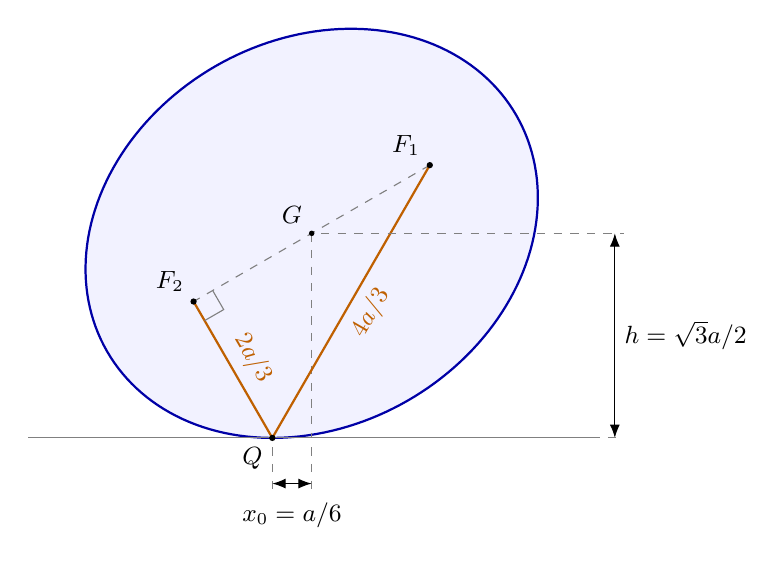
\begin{tikzpicture}[font=\small]
\bodyshape
\draw[gray,dashed](G)--(0,0);
\draw[gray,dashed](Fone)--(Ftwo);
\draw[orange!75!black,thick](Fone)--(Q)node[midway,sloped,below]{$4a/3$};
\draw[orange!75!black,thick](Ftwo)--(Q)node[midway,sloped,above]{$2a/3$};
\dotsGQ
\fill(Fone)circle(.04)node[above left]{$F_1$};
\fill(Ftwo)circle(.04)node[above left]{$F_2$};
\draw[<->](3.85,0)--(3.85,{1.5*sqrt(3)})node[midway,right]{$h=\sqrt3 a/2$};
\draw[gray,dashed](.12,{1.5*sqrt(3)})--(3.96,{1.5*sqrt(3)});
\draw[gray,dashed](3.55,0)--(3.96,0);
\draw[gray,dashed](-.5,-.12)--(-.5,-.65)(0,-.12)--(0,-.65);
\draw[<->](-.5,-.58)--(0,-.58);
\node[below]at(-.25,-.7){$x_0=a/6$};
\draw[gray](Ftwo)++(-60:.28)--++(30:.28)--++(120:.28);
\end{tikzpicture}
\begin{tikzpicture}[font=\small]
\begin{scope}
\bodyshape \dotsGQ
\draw[force](Q)--(-.5,1.3)node[left]{$N$};
\draw[force](G)--(0,1.25)node[right]{$mg$};
\node[above]at(0,5.6){光滑接触：$f=0$};
\end{scope}
\begin{scope}[xshift=8cm]
\bodyshape \dotsGQ
\draw[force](Q)--(-.5,1.3)node[left]{$N$};
\draw[force](G)--(0,1.25)node[right]{$mg$};
\draw[force](Q)--(1.05,0)node[below]{$f$};
\node[above]at(0,5.6){纯滚动：该时刻 $f>0$};
\end{scope}
\end{tikzpicture}
\begin{tikzpicture}[font=\small]
\begin{scope}
\bodyshape \dotsGQ
\fill(Fone)circle(.04)node[above left]{$F_1$};
\draw[velocity](G)--(0,1.3)node[left]{$\boldsymbol v_G$};
\draw[velocity](Fone)--(2.28,{2*sqrt(3)-1.80})node[right]{$\boldsymbol v_{F_1}$};
\draw[gray,dashed](G)--(Q);
\node[above]at(0,5.6){光滑接触：$\dot X=0$};
\end{scope}
\begin{scope}[xshift=8cm]
\bodyshape \dotsGQ
\fill(Fone)circle(.04)node[above left]{$F_1$};
\draw[velocity](G)--(1.65,{1.5*sqrt(3)-.3175})node[below]{$\boldsymbol v_G$};
\draw[velocity](Fone)--(3.06,{2*sqrt(3)-.90})node[right]{$\boldsymbol v_{F_1}$};
\draw[gray,dashed](Q)--(Fone);
\node[below right]at(Q){$\boldsymbol v_Q=0$};
\node[above]at(0,5.6){纯滚动：$\dot X=h\omega$};
\end{scope}
\end{tikzpicture}
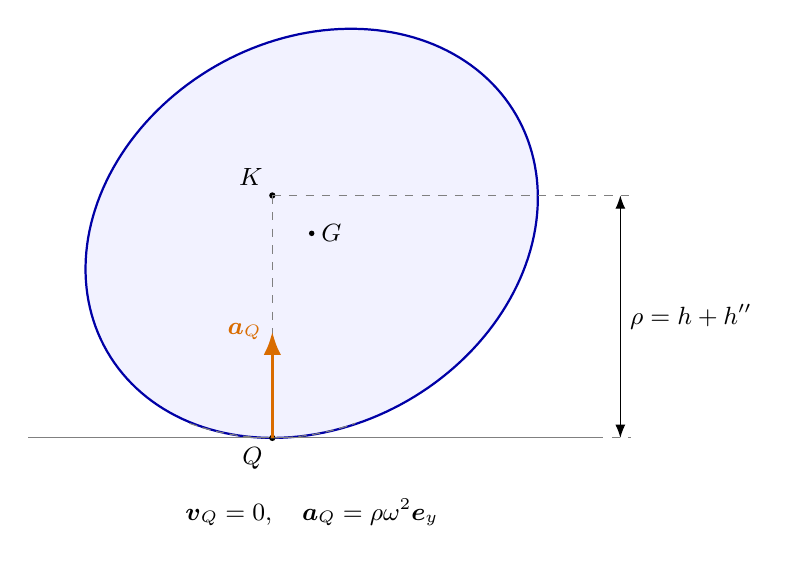
\begin{tikzpicture}[font=\small]
\bodyshape
\coordinate(K)at(-.5,{16/(3*sqrt(3))});
\fill(G)circle(.035)node[right]{$G$};
\fill(Q)circle(.04)node[below left]{$Q$};
\fill(K)circle(.04)node[above left]{$K$};
\draw[gray,dashed](K)--(Q);
\draw[gray,densely dashed]({-.5+(16/(3*sqrt(3)))*cos(250)},{16/(3*sqrt(3))+(16/(3*sqrt(3)))*sin(250)})arc[start angle=250,end angle=290,radius={16/(3*sqrt(3))}];
\draw[force](Q)--(-.5,1.35)node[left]{$\boldsymbol a_Q$};
\draw[gray,dashed](K)--(4.05,{16/(3*sqrt(3))});
\draw[gray,dashed](3.6,0)--(4.05,0);
\draw[<->](3.92,0)--(3.92,{16/(3*sqrt(3))})node[midway,right]{$\rho=h+h''$};
\node[below]at(0,-.65){$\boldsymbol v_Q=0,\quad \boldsymbol a_Q=\rho\omega^2\boldsymbol e_y$};
\end{tikzpicture}
\end{document}
